\section{Programm}\label{Programm}
Um die Methoden der Threads in einer realen Situation zu nutzen, habe ich mich entschlossen ein Programm, welches stark von Threads profitieren kann, zu programmieren.  

Ich habe mich für ein Programm entschieden, mit dem man ein gewünschtes Bild mit vielen weiteren Bildern rekonstruieren kann. Es wird demnach ein Mosaik aus Bildern erstellt.

\begin{figure}[h]
    \centering
    \subfloat[\centering Eingabe]{
        
\includegraphics[height=5cm]{images/Source_100x100.pdf}
    }
    \subfloat[\centering Ausgabe]{
        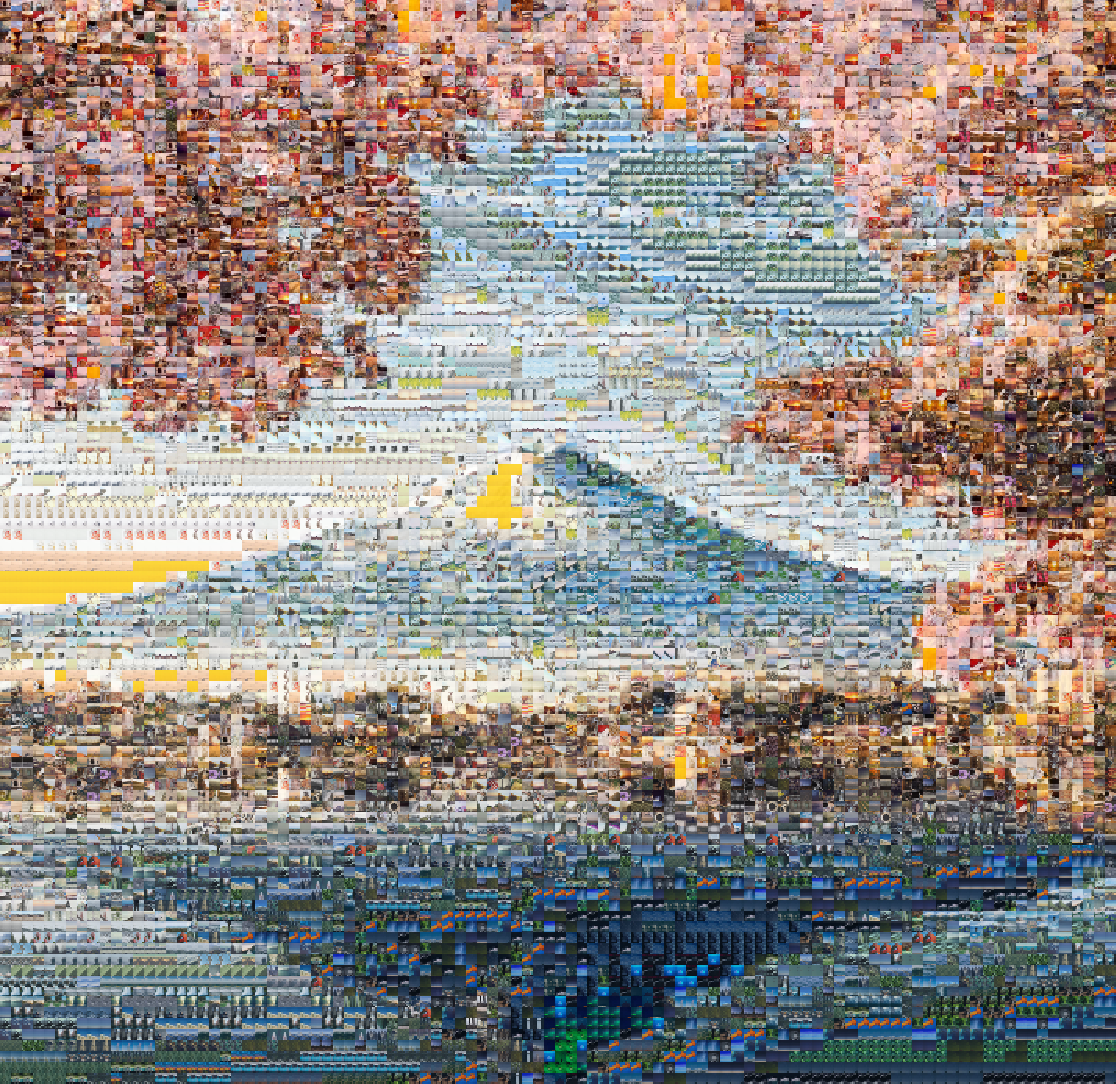
\includegraphics[height=5cm]{images/Render_100x100.pdf}
    }
    \caption[Programm Funktion]{Funktionsweise des Programmes}
\end{figure}

Die Anwendung von Threads kommt in dem Programm an vielen Stellen vor. Im folgenden werde ich mich auf die Algorithmen der Bildanalyse und Verarbeitung beziehen. Andere Aspekte, wie die Implementation des Testmodus und anderen Funktionen, die in der App vorhanden sind, werden kurz im Anhang erwähnt.